\documentclass[paper=a4, fontsize=11pt]{scrartcl} % KOMA-article class

%-------------------------------------------------
%   THEMES, PACKAGES, CUSTOM COMMANDS
%-------------------------------------------------
\usepackage{blindtext}
\usepackage[english]{babel}                             % English language/hyphenation
\usepackage[protrusion=true,expansion=true]{microtype}  % Better typography
\usepackage{amsmath,amsfonts,amsthm}                    % Math packages
\usepackage[pdftex]{graphicx}                           % Enable pdflatex
\usepackage[export]{adjustbox}
\usepackage[svgnames]{xcolor}                           % Enabling colors by their 'svgnames'
\usepackage[hang, small,labelfont=bf,up,textfont=it,up]{caption} % Custom captions under/above floats
\usepackage{subcaption}
\usepackage{caption}
\usepackage{epstopdf}       % Converts .eps to .pdf
%\usepackage{subfig}         % Subfigures
\usepackage{booktabs}       % Nicer tables
\usepackage{fix-cm}         % Custom fontsizes
\usepackage{listings}
\usepackage{soul}
\usepackage{float}

\usepackage{hyperref}

\usepackage[foot=30pt,margin=1in]{geometry}

% Custom sectioning (sectsty package)
\usepackage{sectsty}
\allsectionsfont{
    \usefont{OT1}{phv}{b}{n}    % bch-b-n: CharterBT-Bold font
}
\sectionfont{
    \usefont{OT1}{phv}{b}{n}
}

% Custom colors
\definecolor{brsugrey}{rgb}{0.9, 0.9, 0.9}
\definecolor{brsublue}{rgb}{0, 0.594, 0.949}

%
\newcommand{\upperRomannumeral}[1]{\uppercase\expandafter{\romannumeral#1}}

% Creating an initial of the very first character of the content
\usepackage{lettrine}
\newcommand{\initial}[1]{%
    \lettrine[lines=3,lhang=0.3,nindent=0em]{
        \color{brsublue}
        {\textsf{#1}}}{}}

%-------------------------------------------------
%   COMMON INFO
%-------------------------------------------------
\newcommand{\hmwkTitle}{Week \upperRomannumeral{6} report}
\newcommand{\hmwkDueDate}{Monday, November 14, 2016}
\newcommand{\hmwkClass}{Scientific Evaluation and Experimentation}
\newcommand{\hmwkClassShort}{SEE WS2016}
\newcommand{\hmwkAuthorFullName}{Minh H. Nguyen \& Bach D. Ha}
\newcommand{\hmwkAuthorLastName}{Nguyen \& Ha}
\newcommand{\hmwkAuthorEmail}{minh.nguyen@smail.inf.h-brs.de\\
                              bach.ha@smail.inf.h-brs.de}
\newcommand{\hmwkAuthorInstitute}{BRS University of Applied Sciences}

%-------------------------------------------------
%   HEADERS & FOOTERS
%-------------------------------------------------
\usepackage{fancyhdr}
\pagestyle{fancy}
\usepackage{lastpage}
% Header (empty)
\lhead{}
\chead{}
\rhead{}
% Footer (you may change this to your own needs)
\lfoot{\footnotesize
    \texttt{\hmwkClassShort} ~
    \textbullet ~ \hmwkAuthorLastName ~
    \textbullet ~ \hmwkTitle}
\cfoot{}
\rfoot{\footnotesize page \thepage\ of \pageref{LastPage}}  % "Page 1 of 2"
\renewcommand{\headrulewidth}{0.0pt}
\renewcommand{\footrulewidth}{0.4pt}

%-------------------------------------------------
%   TITLE & AUTHOR
%-------------------------------------------------
\usepackage{titling}

\newcommand{\HorRule}{\color{brsublue}% Creating a horizontal rule
    \rule{\linewidth}{1pt}%
    \color{black}
}

% Title
\pretitle{
    \vspace{-30pt}
    \begin{flushleft}
        \HorRule
        \fontsize{22}{22} \usefont{OT1}{phv}{b}{n} \color{gray} \selectfont
}
\title{\hmwkClass \\
       \hmwkTitle}
\posttitle{
    \par
    \end{flushleft}
    \vskip 0.5em
}

% Author
\preauthor{
    \begin{flushleft}
        \large \lineskip 0.25em
        \usefont{OT1}{phv}{b}{sl} \color{brsublue}}

\author{\hmwkAuthorFullName}

\postauthor{
        \footnotesize
        \usefont{OT1}{phv}{m}{sl} \color{Black}
        \\\hmwkAuthorInstitute
        \\\hmwkAuthorEmail
        \par
    \end{flushleft}
    \HorRule}

% Date
\date{\hmwkDueDate}

%-------------------------------------------------
%   BEGIN
%-------------------------------------------------
\begin{document}
    \maketitle
    \thispagestyle{fancy} % Enabling the custom headers/footers for the first page

\section{AICISS experiment}
    \subsection{Lab configuration}
        \begin{itemize}
            \item The lab's size is 3m x 7m.
            \item The ground area is divided into 4 parts corresponding to each of 4 cameras.
            \item There is an error in the calibration between cameras, thus experiments are carried out in the region of only one camera, as much as possible.
        \end{itemize}

    \subsection{Experiments}
        \begin{itemize}
            \item Before the experiment, the robot's battery is fully charged to avoid change in the trajectory, which is caused by voltage drop.
            \item The marker is adjust so that it is as parallel to the floor as possible.
            \item During the experiment, robot's location is recorded during 5 different motions: Straight, left, slight left, right, and slight right.
            \item Straight motion: To avoid changing camera region, robot is running along the 3m width side of the lab. After each run, the robot is picked up and placed at the previous starting location. This experiment is carried out 5 times to get enough data.
            \item Left/Right motion: The trajectories of these motions are only inside the region of one camera, thus it is left to run in circle for about 5 minutes.
            \item Slight left/ Slight right motion: the robot is left to run in circle for about 5m. Because the trajectories of these motions are too large for one camera region, the output data exhibits systematic offset in certain part of the trajectory.
            \item In all experiments, the recording process was started only when the robot is moving. The recording is stopped a little before the robot stop. This help eliminate the recording of robot location when it is not moving.  
        \end{itemize}

    \begin{figure}[H]
        \begin{center}
            \setlength{\fboxsep}{0.5pt} %
            \setlength{\fboxrule}{0.5pt}
            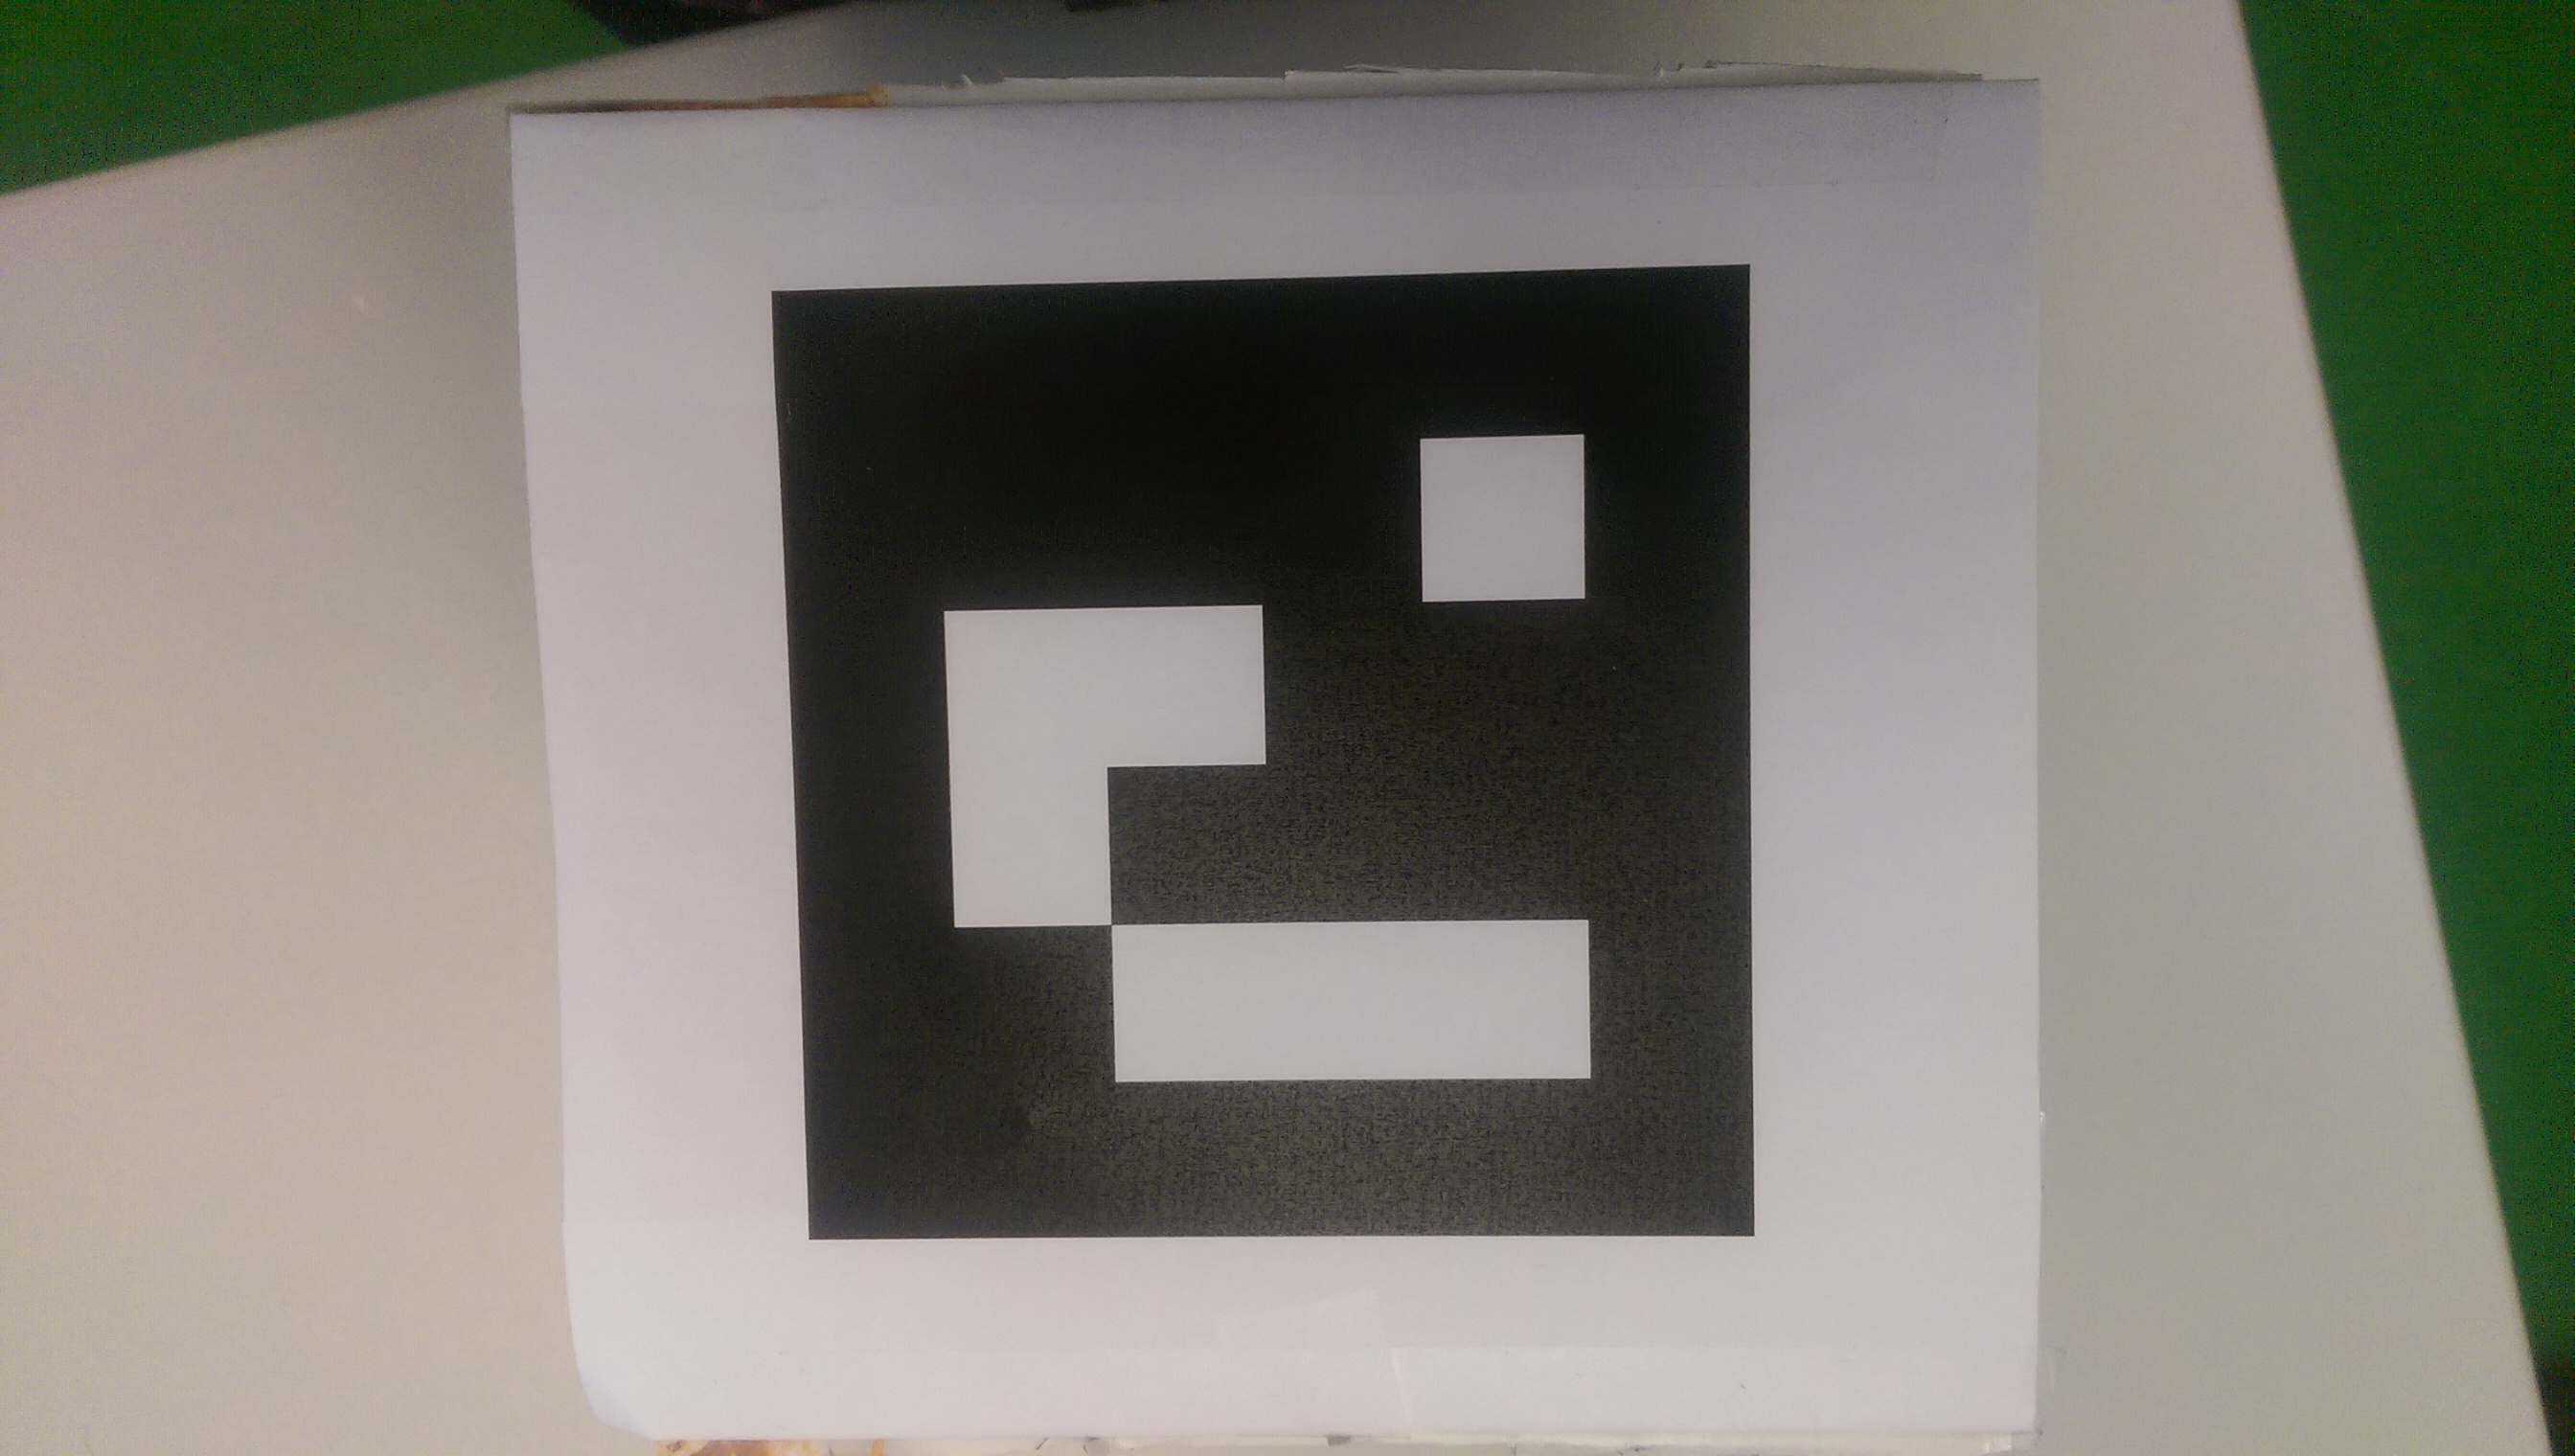
\includegraphics[width=12cm,fbox]{images/marker.jpg}
            \caption{Marker for robot localization.}
        \end{center}
    \end{figure}

    \begin{figure}[H]
        \begin{center}
            \setlength{\fboxsep}{0.5pt} %
            \setlength{\fboxrule}{0.5pt}
            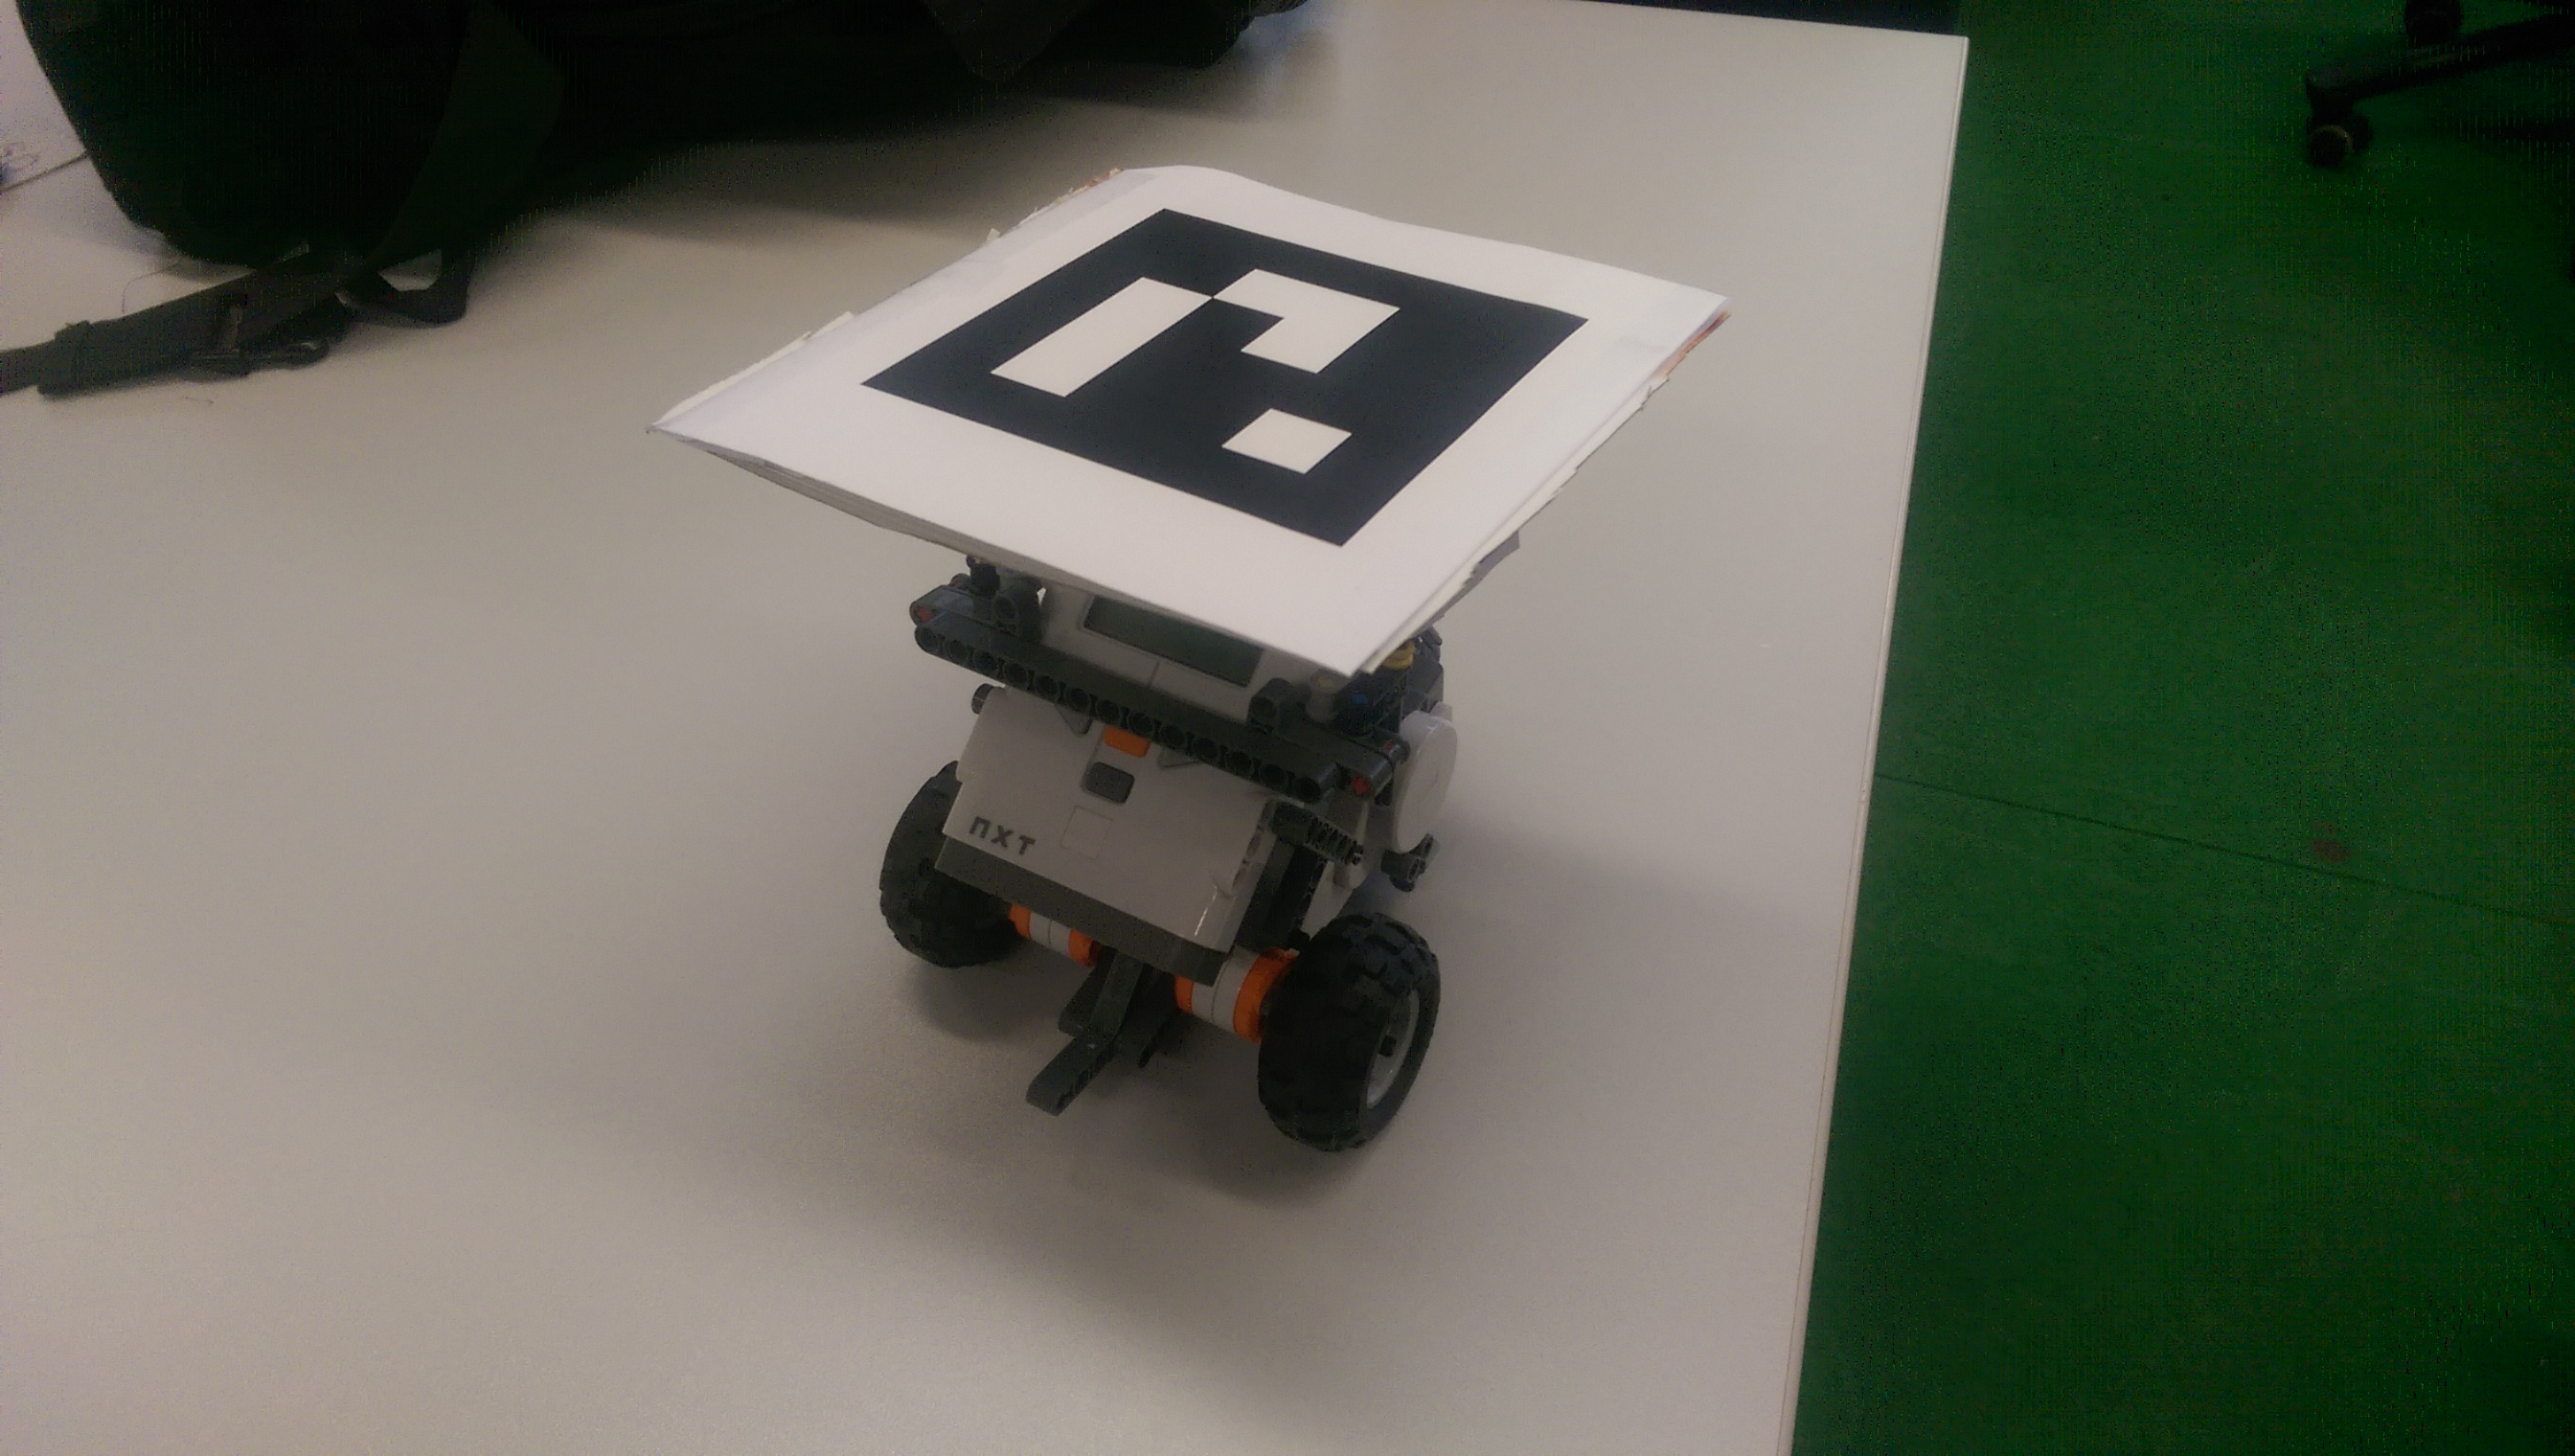
\includegraphics[width=12cm,fbox]{images/marker_robot.jpg}
            \caption{Marker mounted on the robot.}
        \end{center}
    \end{figure}

\section{Motion Model Sampling}
    \begin{itemize}
        \item To perform the optimization, the whole recorded trajectories are divided into several smaller sequences.
        \item Each sequence represents one experiment similar each hand measured experiment.
        \item Each sequence contains all data points in a window of 6 seconds.
        \item Each data point consists of a time stamp (in millisecond), name of observing camera, XY coordinate (in mm), and theta (in radian). Sample of data can be seen in figure \ref{Raw_data}
        \item Plot of raw data can be seen in figure 4,5,6,7, and 8.
    \end{itemize}

    \begin{figure}[H]
        \begin{center}
            \setlength{\fboxsep}{0.5pt} %
            \setlength{\fboxrule}{0.5pt}
            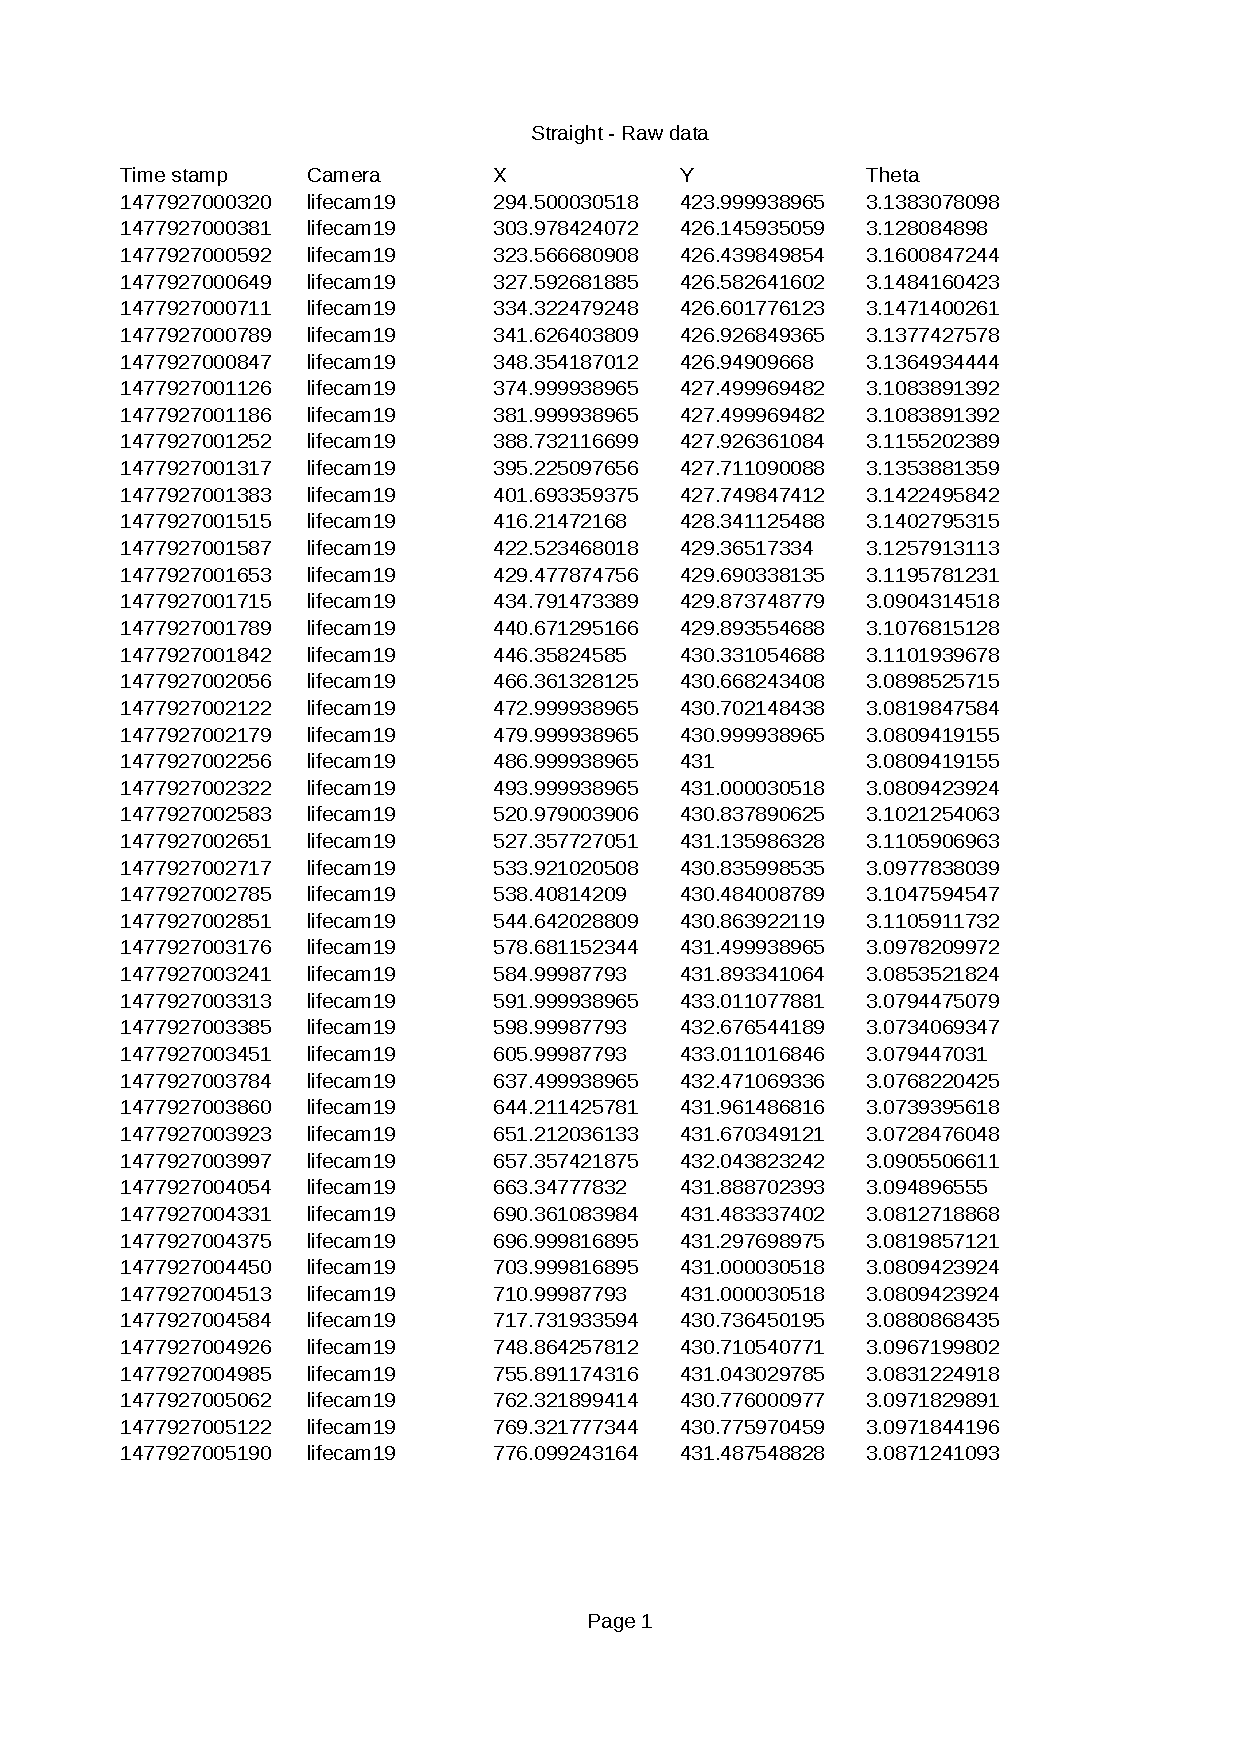
\includegraphics[width=12cm,fbox]{images/Raw_data}
            \caption{Raw data sample}
            \label{Raw_data}
        \end{center}
    \end{figure}

    \begin{figure}[H]
        \begin{center}
            \setlength{\fboxsep}{0.5pt} %
            \setlength{\fboxrule}{0.5pt}
            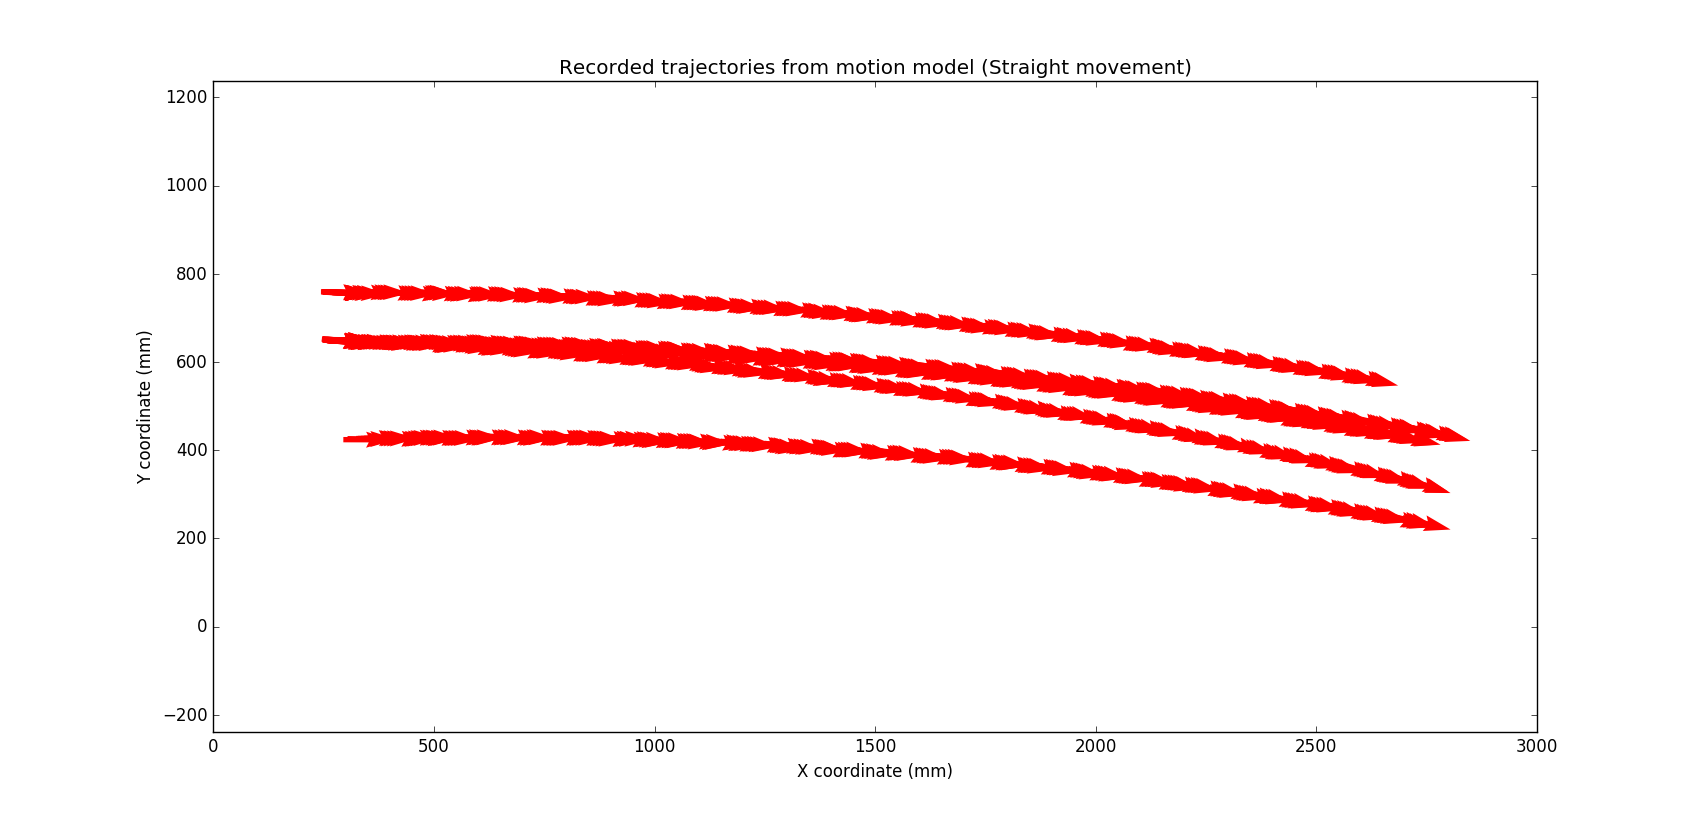
\includegraphics[width=\linewidth,fbox]{images/raw_straight.png}
            \caption{Sampled poses of the LeJOS robot going straight.}
        \end{center}
    \end{figure}

    \begin{figure}[H]
        \begin{center}
            \setlength{\fboxsep}{0.5pt} %
            \setlength{\fboxrule}{0.5pt}
            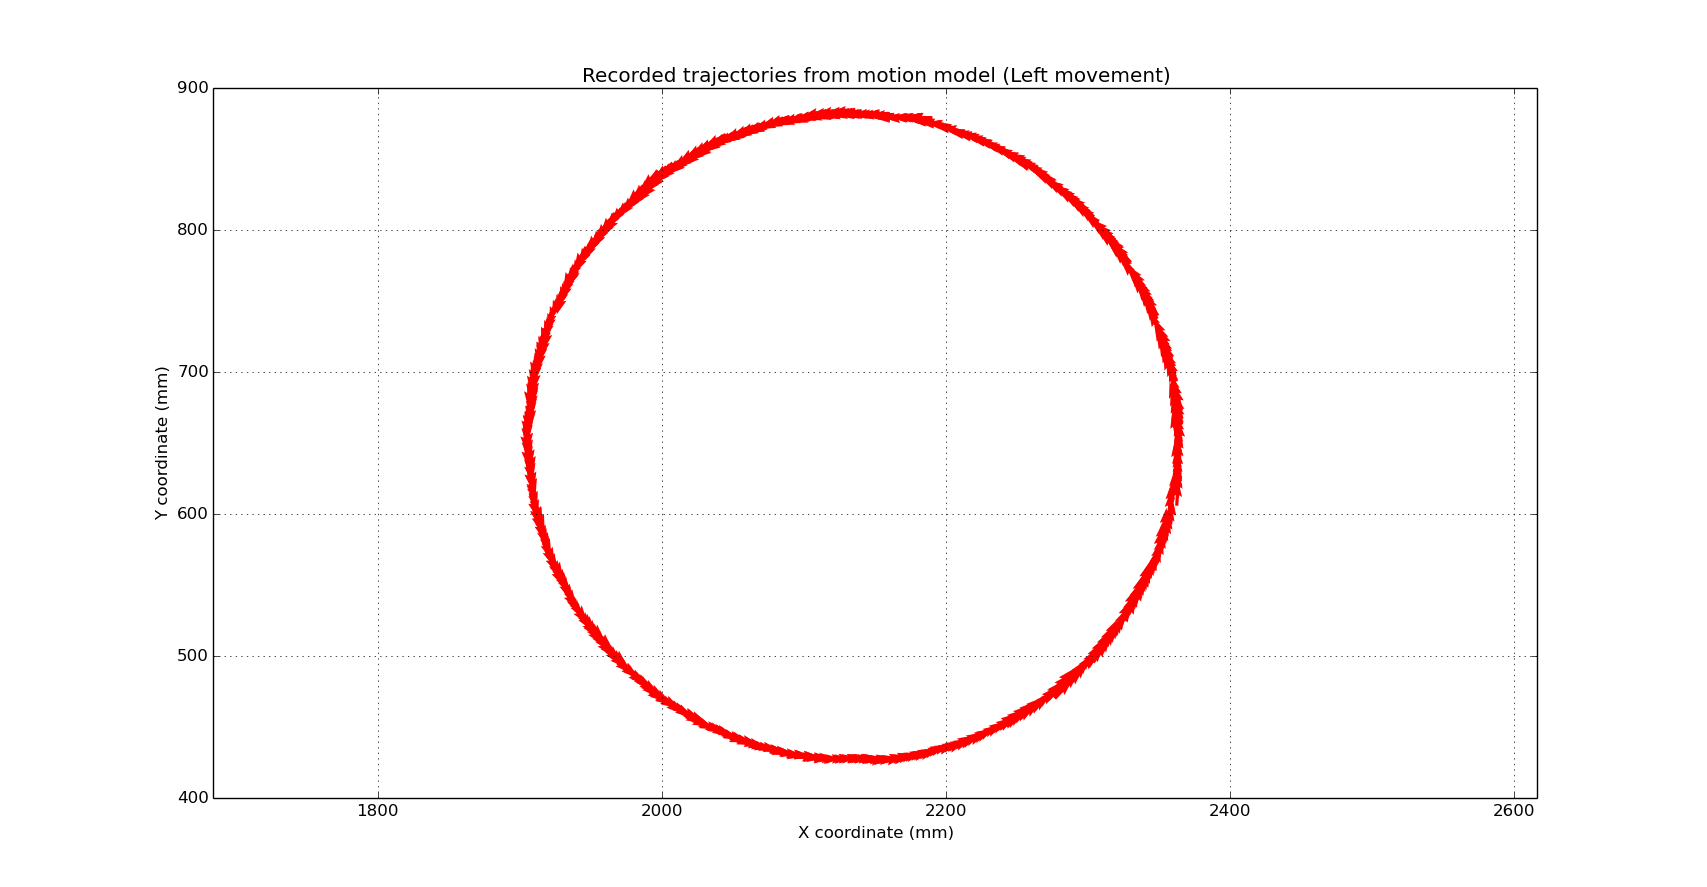
\includegraphics[width=\linewidth,fbox]{images/raw_left.png}
            \caption{Sampled poses of the LeJOS robot going left.}
        \end{center}
    \end{figure}

    \begin{figure}[H]
        \begin{center}
            \setlength{\fboxsep}{0.5pt} %
            \setlength{\fboxrule}{0.5pt}
            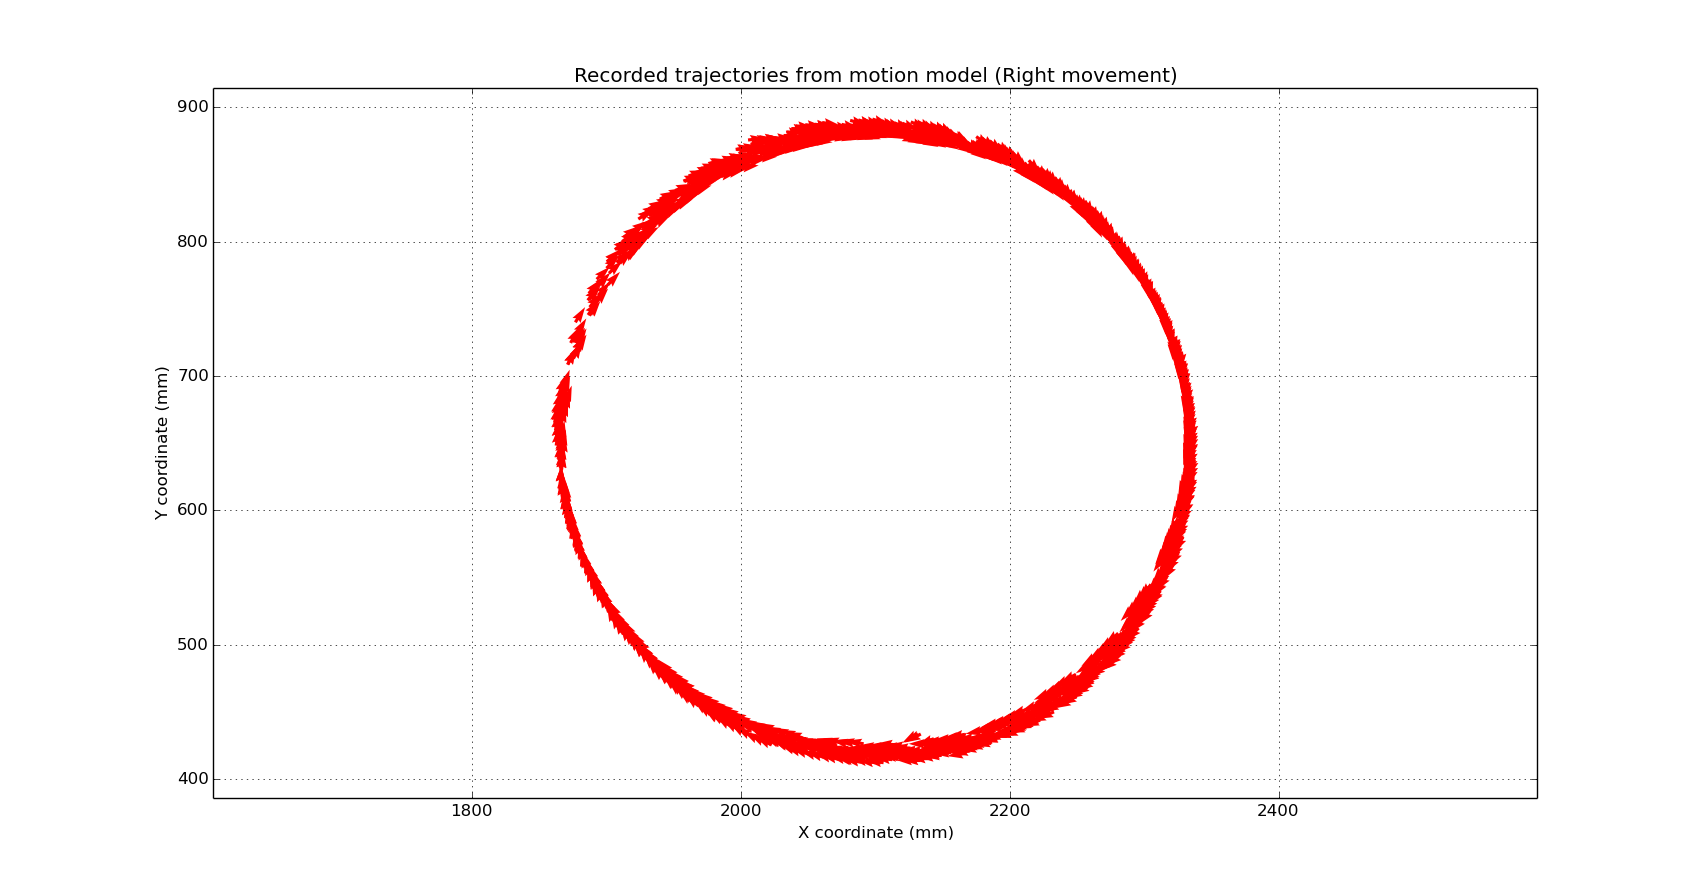
\includegraphics[width=\linewidth,fbox]{images/raw_right.png}
            \caption{Sampled poses of the LeJOS robot going right.}
        \end{center}
    \end{figure}

    \begin{figure}[H]
        \begin{center}
            \setlength{\fboxsep}{0.5pt} %
            \setlength{\fboxrule}{0.5pt}
            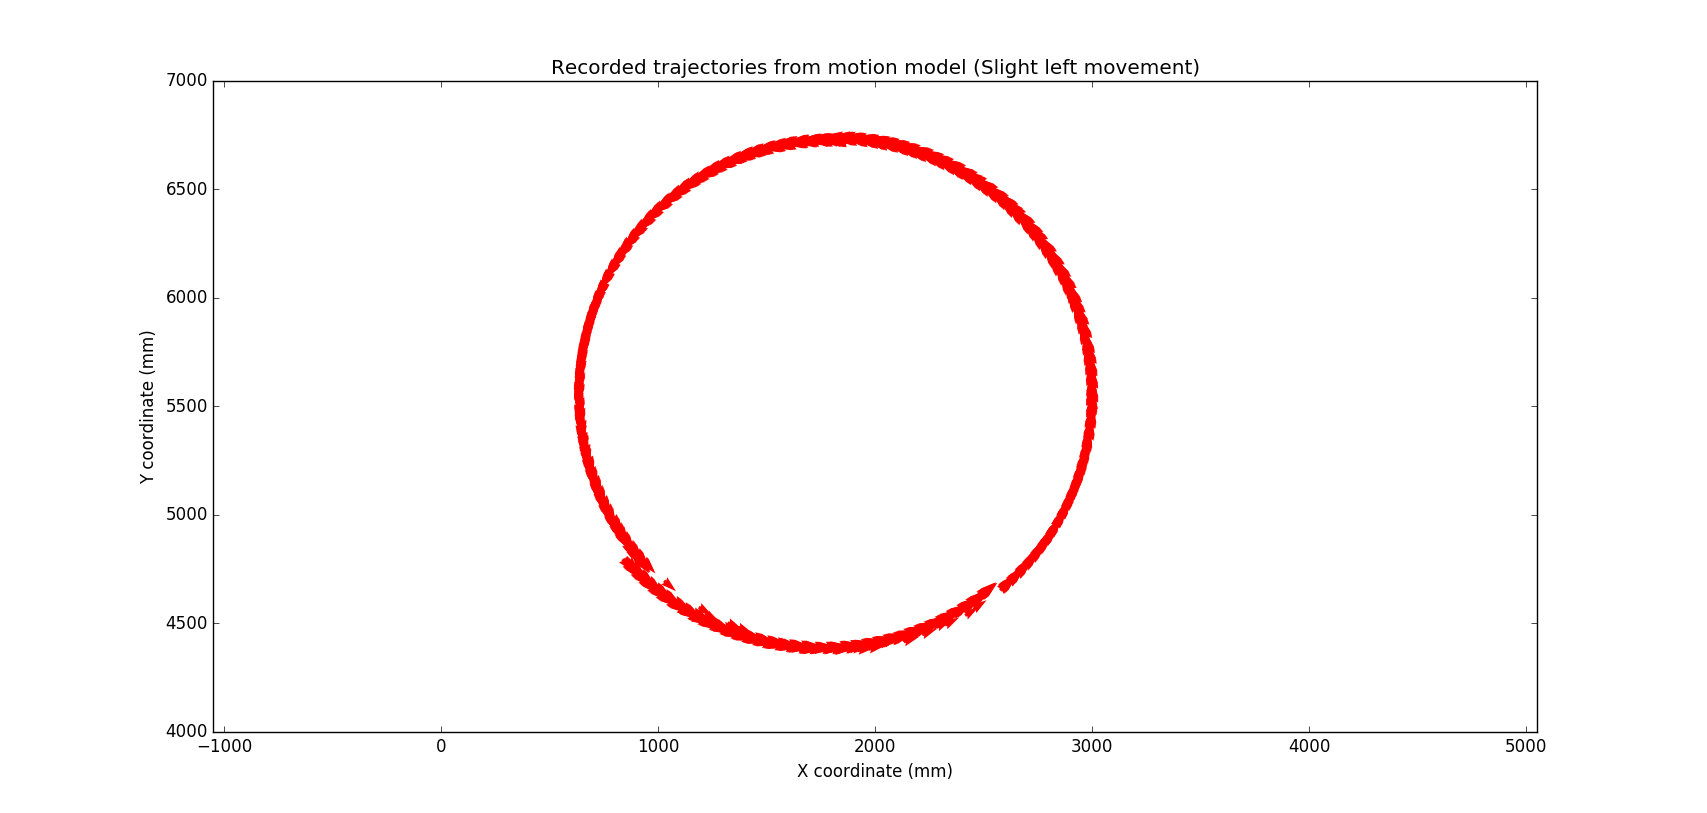
\includegraphics[width=\linewidth,fbox]{images/raw_slightLeft.png}
            \caption{Sampled poses of the LeJOS robot going slight left.}
        \end{center}
    \end{figure}

    \begin{figure}[H]
        \begin{center}
            \setlength{\fboxsep}{0.5pt} %
            \setlength{\fboxrule}{0.5pt}
            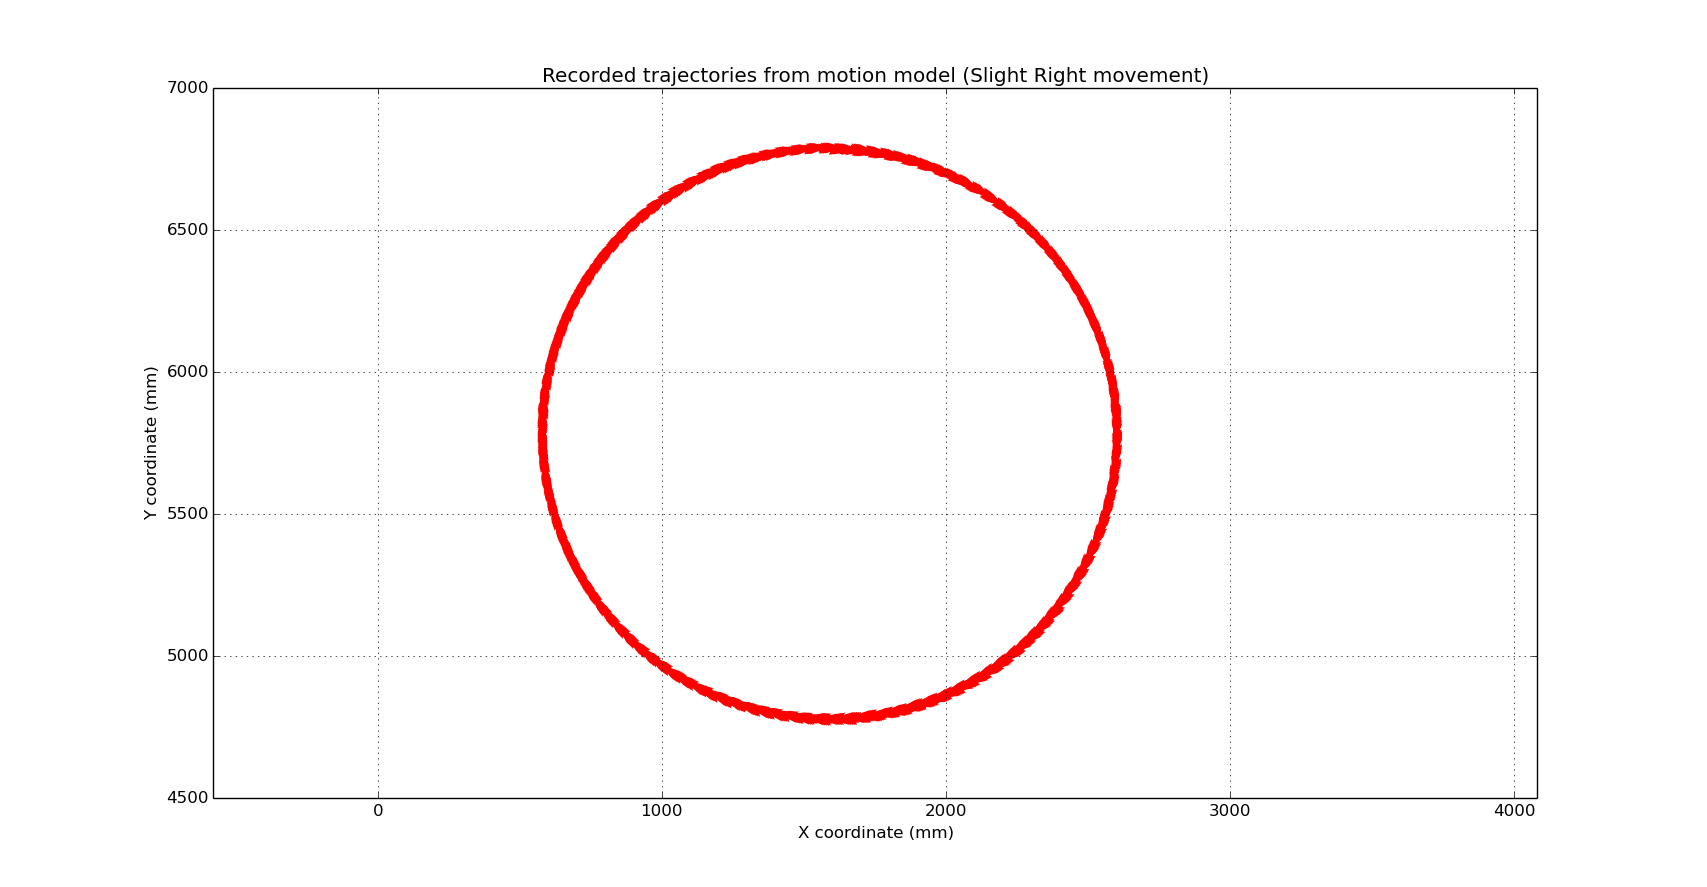
\includegraphics[width=\linewidth,fbox]{images/raw_slightRight.png}
            \caption{Sampled poses of the LeJOS robot going slight right.}
        \end{center}
    \end{figure}

    \subsection{Parameters calculation}
    \begin{itemize}
        \item Alphas are parameters of the velocity motion model introduced by Thrun \cite{Thrun}.
        \item The probability of the location of the robot can be calculated from the previous location and the velocity command.
        \[
        P(x_t \mid x_(t-1),u_t) = \mathcal{N}(0,\alpha_1 v^2 + \alpha_2 \omega^2) \cdot \mathcal{N}(0,\alpha_3 v^2 + \alpha_4 \omega^2) \cdot \mathcal{N}(0,\alpha_5 v^2 + \alpha_6 \omega^2) 
        \]
        \item Data collected from experiments are robot poses with time stamp. Velocity command is also available.
        \item To find alphas, the $P(x_t \mid x_(t-1),u_t)$ must be maximized using collected poses and known velocity command.
        \item Following the Bayes' rule:
        \[
        P(\alpha \mid X) = \cfrac{P(X \mid \alpha) P(\alpha)}{P(X)}
        \]
        \item P(X) is independence of $\alpha$, and assuming that $P(\alpha)$ is a uniform distribution. It means that maximizing $P(X \mid \alpha)$ will lead to maximization of $P(\alpha \mid X)$
        \[
        P(x \mid \alpha) = \mathcal{N}(0,\alpha_1 v^2 + \alpha_2 \omega^2) \cdot \mathcal{N}(0,\alpha_3 v^2 + \alpha_4 \omega^2) \cdot \mathcal{N}(0,\alpha_5 v^2 + \alpha_6 \omega^2)
        \]
        \[
        = \cfrac{1}{\sqrt{2\pi} \sqrt{\alpha_1 v^2 + \alpha_2 \omega^2}} \cdot exp(-\cfrac{1}{2}\cfrac{v - \hat{v}}{\alpha_1 v^2 + \alpha_2 \omega^2}) \cdot \cfrac{1}{\sqrt{2\pi} \sqrt{\alpha_3 v^2 + \alpha_4 \omega^2}} \cdot exp(-\cfrac{1}{2}\cfrac{\omega - \hat{\omega}}{\alpha_3 v^2 + \alpha_4 \omega^2}) 
        \]
        \[	
        \cdot \cfrac{1}{\sqrt{2\pi} \sqrt{\alpha_5 v^2 + \alpha_6 \omega^2}} \cdot exp(-\cfrac{1}{2}\cfrac{\hat{\gamma}}{\alpha_5 v^2 + \alpha_6 \omega^2})
        \]
        
        \item To simplify calculation, the log likelihood is maximized instead.
        \[
        ln P(x \mid \alpha) = - \cfrac{1}{2}( 3ln(2\pi) + ln(\alpha_1 v^2 + \alpha_2 \omega^2) + \cfrac{v - \hat{v}}{\alpha_1 v^2 + \alpha_2 \omega^2} + ln(\alpha_3 v^2 + \alpha_4 \omega^2) + \cfrac{\omega - \hat{\omega}}{\alpha_3 v^2 + \alpha_4 \omega^2} 
        \]
        \[
        + ln(\alpha_5 v^2 + \alpha_6 \omega^2) + \cfrac{\hat{\gamma}}{\alpha_5 v^2 + \alpha_6 \omega^2})
        \]
        \item Optimizing the $ln P(x \mid \alpha)$ using its derivatives with respect to each $\alpha$ result in the value of 6 alphas.
    \end{itemize}

    \begin{figure}[h!]
        \centering
        \def\arraystretch{1.5}
        \begin{tabular}{|c|c|}
            \hline
            Parameter & Value \\
            \hline
            $\alpha_1$ & $1.18337602\times 10 ^{-2}$ \\
            $\alpha_2$ & $4.50020855\times 10 ^{-6}$ \\
            $\alpha_3$ & $7.97143571\times 10 ^{-5}$ \\
            $\alpha_4$ & $6.31096021\times 10 ^{-6}$ \\
            $\alpha_5$ & $7.37806701\times 10 ^{-5}$ \\
            $\alpha_6$ & $6.78659476\times 10 ^{-6}$ \\
            \hline
        \end{tabular}
        \captionof{table}{Calculated parameters of the motion model}
    \end{figure}

    The parameters are then used to sample poses and compare with observed data.

    \begin{figure}[H]
        \centering
        \begin{minipage}{\textwidth}
            \centering
            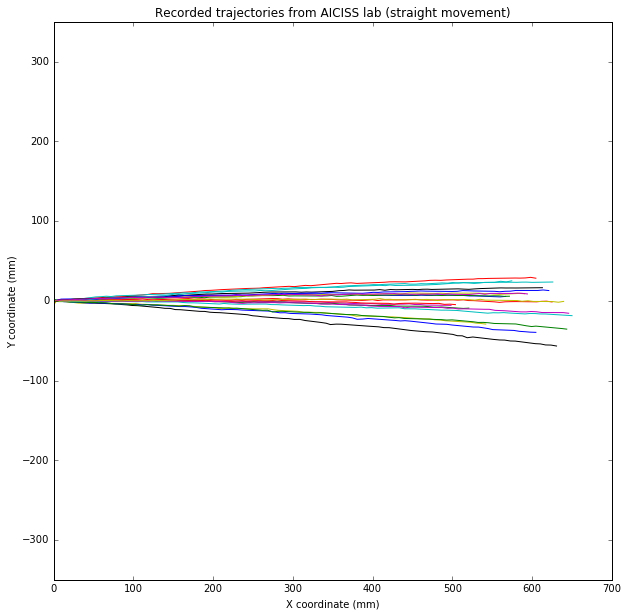
\includegraphics[width=1\textwidth]{images/recorded_poses_straight.png} % first figure itself
            \caption{Recorded poses of the LeJOS robot going straight.}
        \end{minipage}\hfill
        \begin{minipage}{\textwidth}
            \centering
            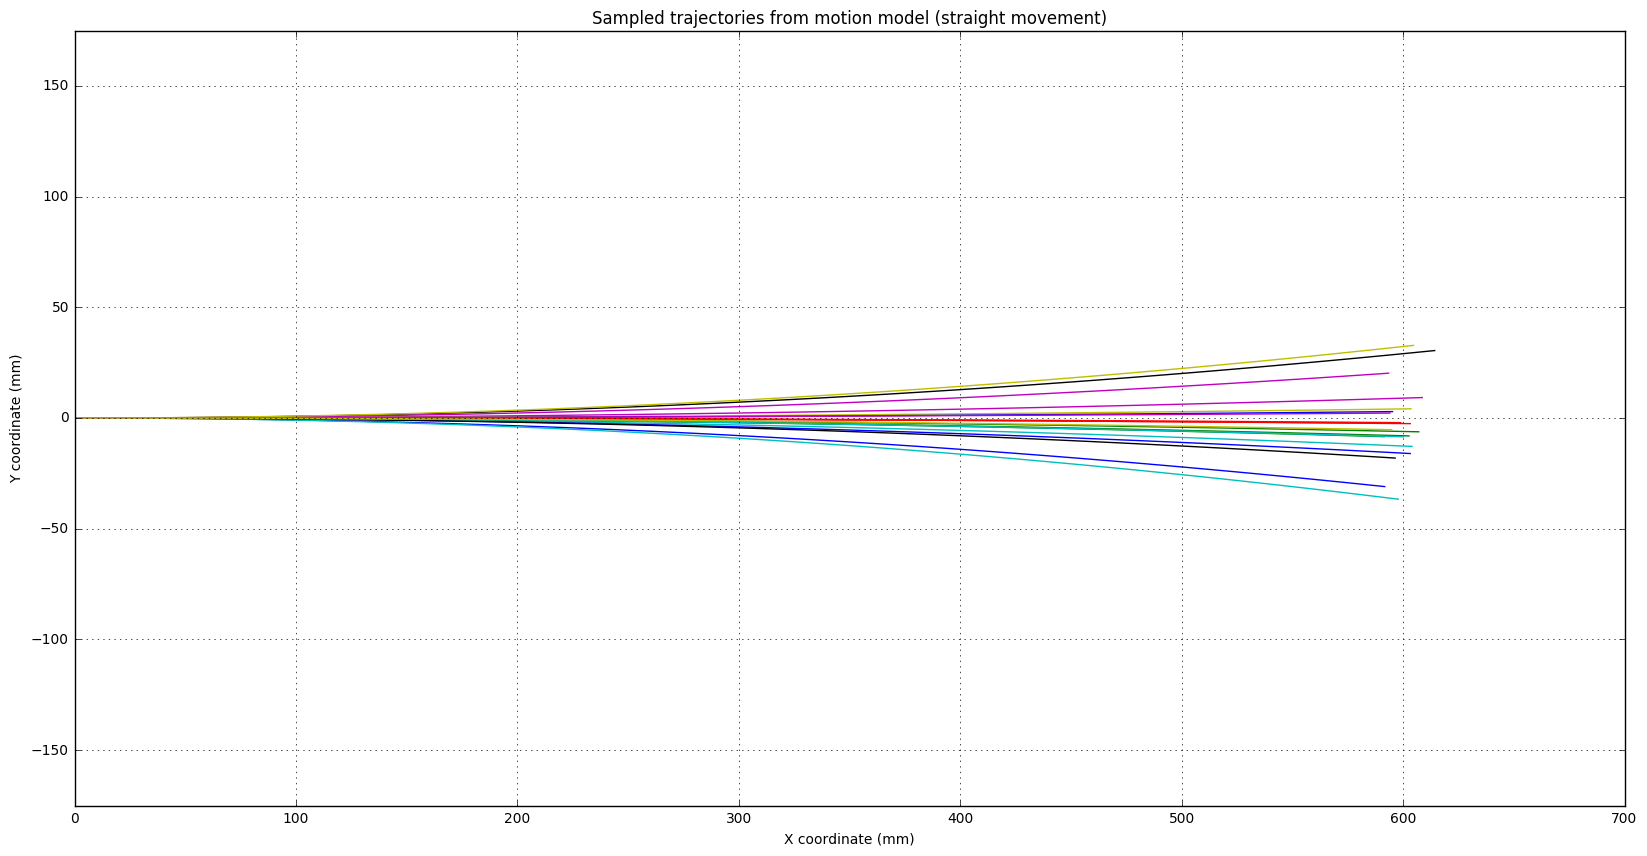
\includegraphics[width=1\textwidth]{images/sampled_poses_straight.png} % second figure itself
            \caption{Sampled poses of the LeJOS robot going straight.}
        \end{minipage}
    \end{figure}

    \begin{figure}[H]
        \centering
        \begin{minipage}{0.5\textwidth}
            \centering
            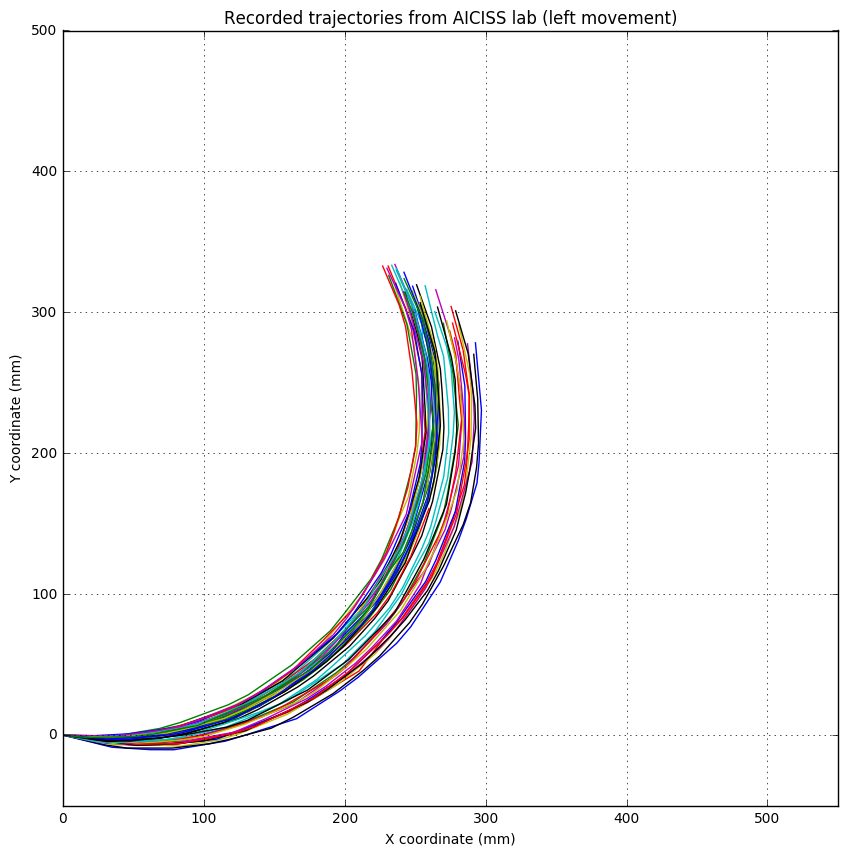
\includegraphics[width=1\textwidth]{images/recorded_poses_left.png} % first figure itself
            \caption{Recorded poses of the LeJOS robot going left.}
        \end{minipage}\hfill
        \begin{minipage}{0.5\textwidth}
            \centering
            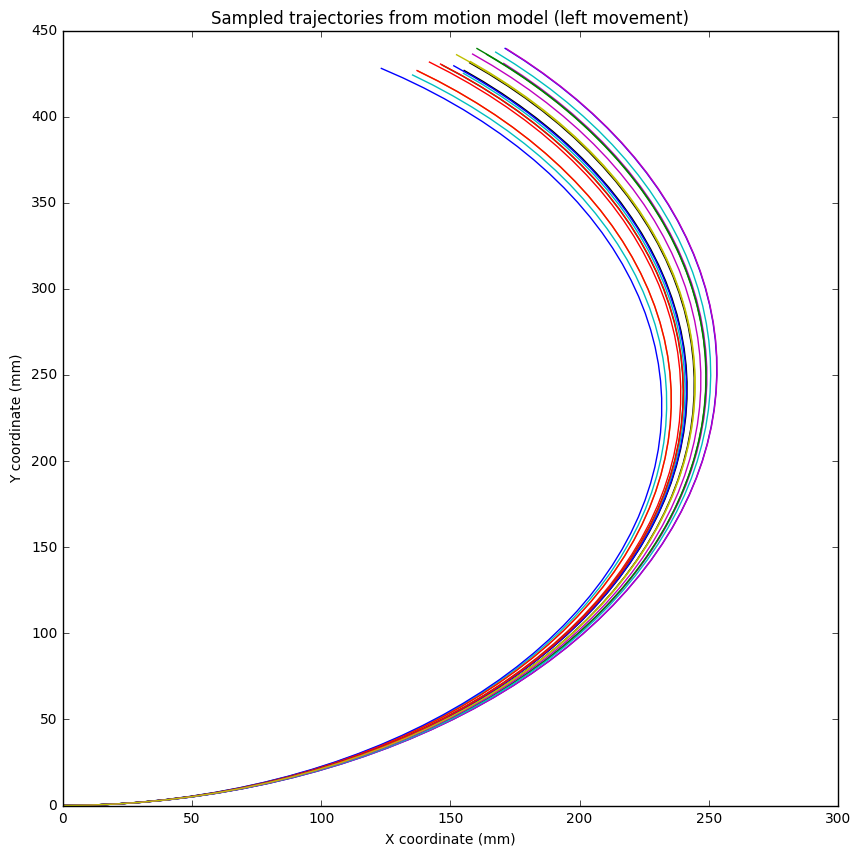
\includegraphics[width=1\textwidth]{images/sampled_poses_left.png} % second figure itself
            \caption{Sampled poses of the LeJOS robot going left.}
        \end{minipage}
    \end{figure}

    \begin{figure}[h!]
        \centering
        \begin{minipage}{0.5\textwidth}
            \centering
            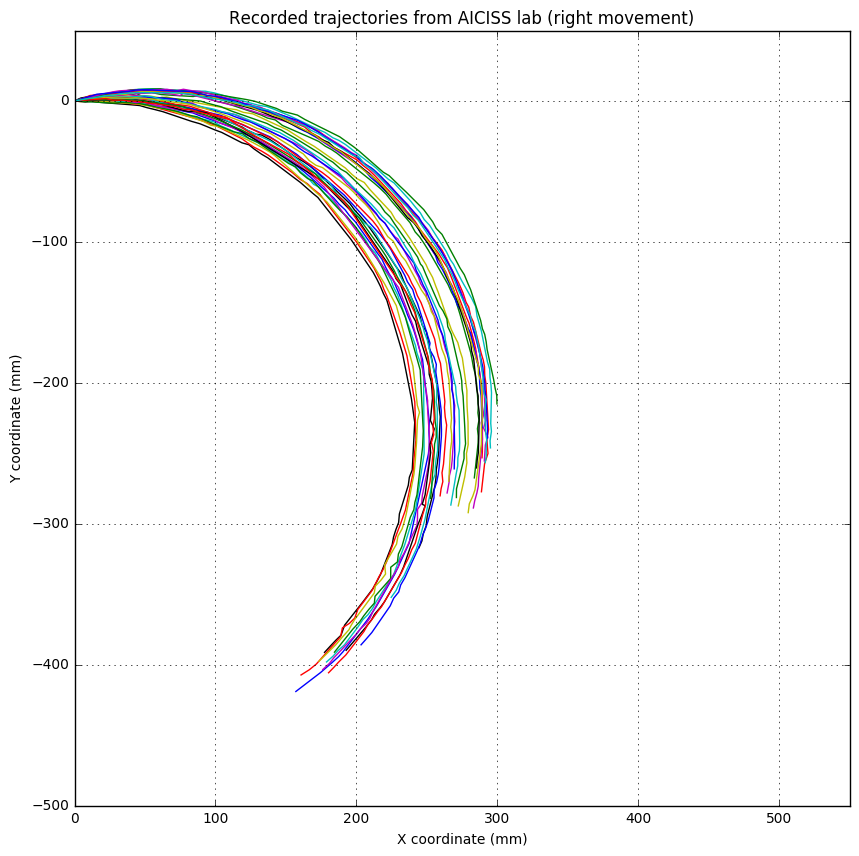
\includegraphics[width=1\textwidth]{images/recorded_poses_right.png} % first figure itself
            \caption{Recorded poses of the LeJOS robot going right.}
        \end{minipage}\hfill
        \begin{minipage}{0.5\textwidth}
            \centering
            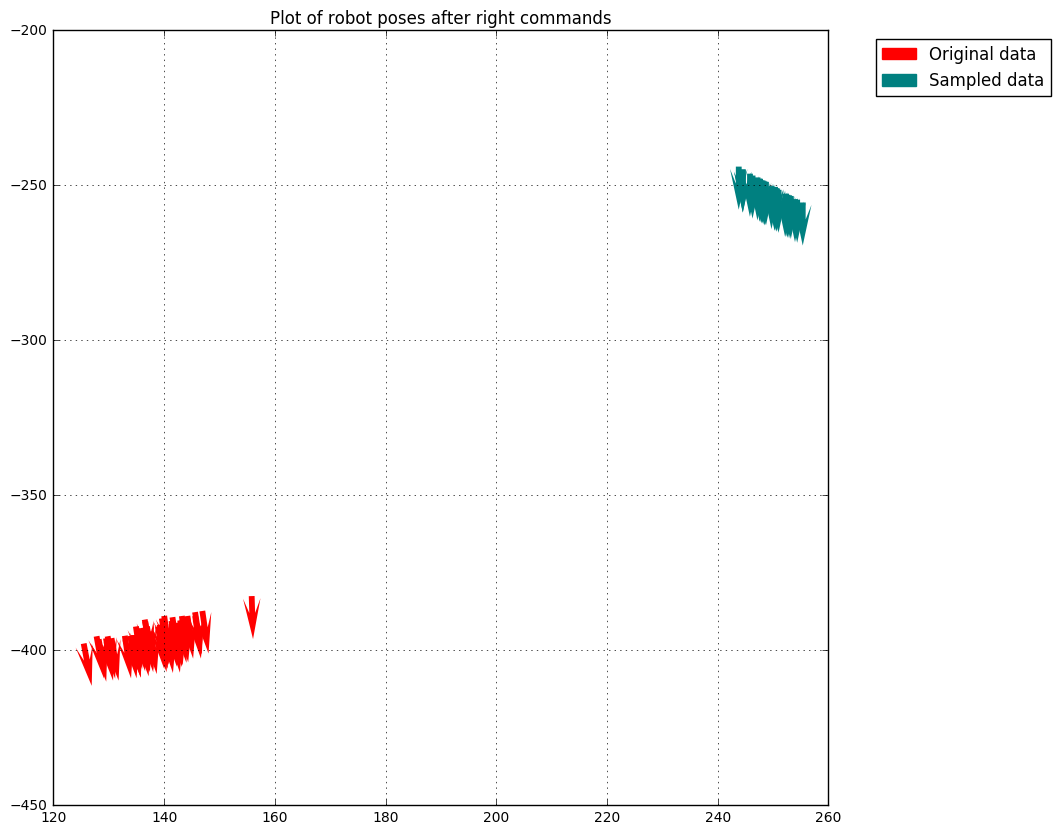
\includegraphics[width=1\textwidth]{images/sampled_poses_right.png} % second figure itself
            \caption{Sampled poses of the LeJOS robot going right.}
        \end{minipage}
    \end{figure}

    \begin{figure}[H]
    \centering
    \begin{minipage}{\textwidth}
        \centering
        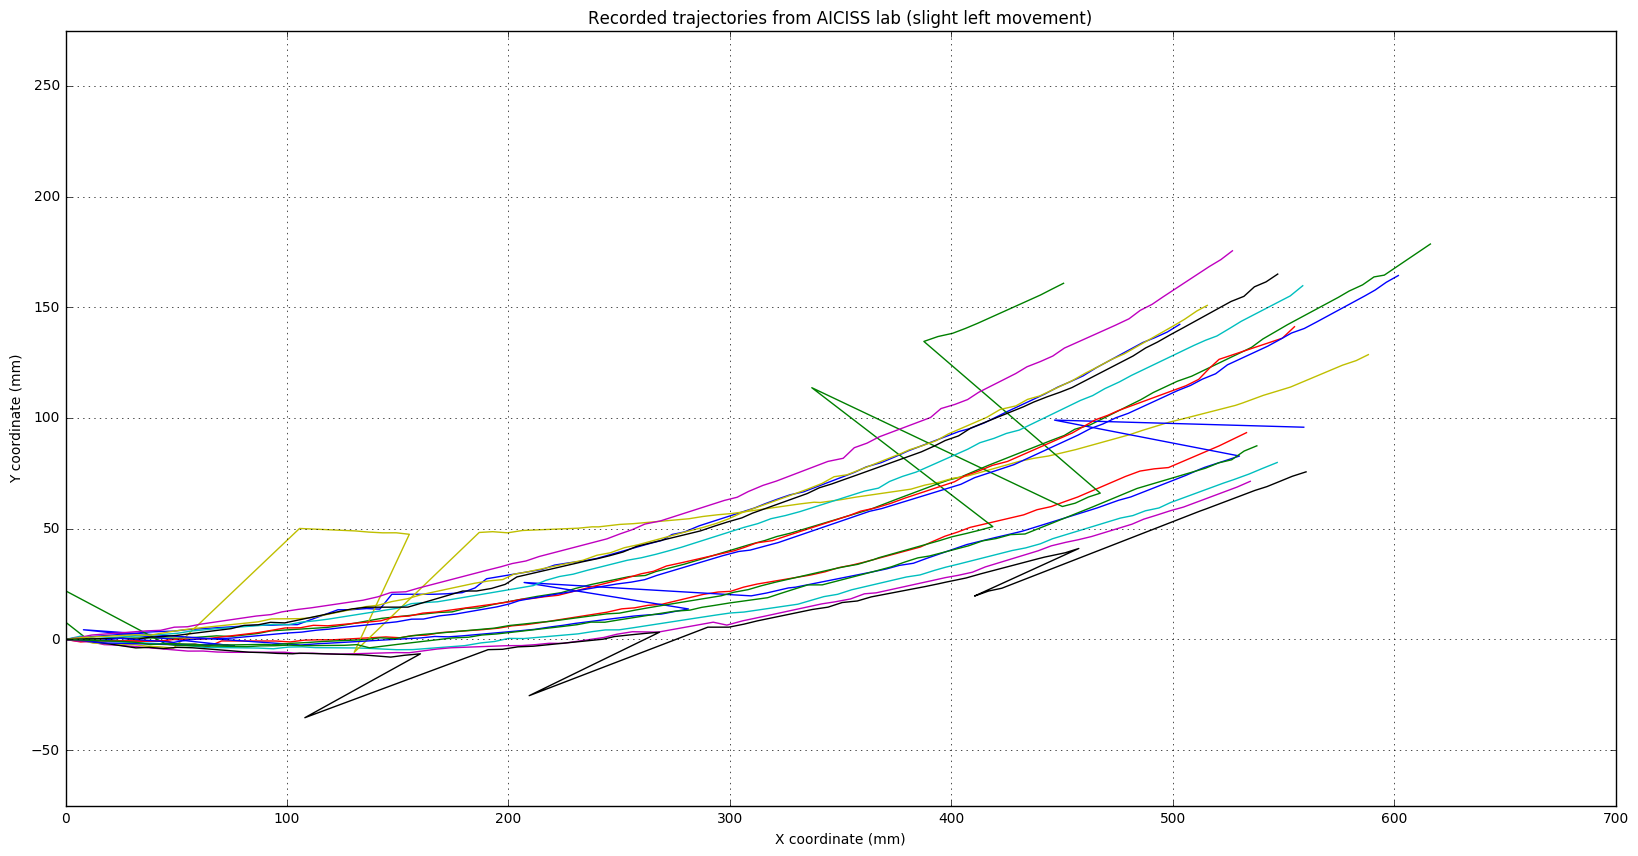
\includegraphics[width=\textwidth]{images/recorded_poses_slight_left.png} % first figure itself
        \caption{Recorded poses of the LeJOS robot going slight left.}
    \end{minipage}\hfill
    \begin{minipage}{\textwidth}
        \centering
        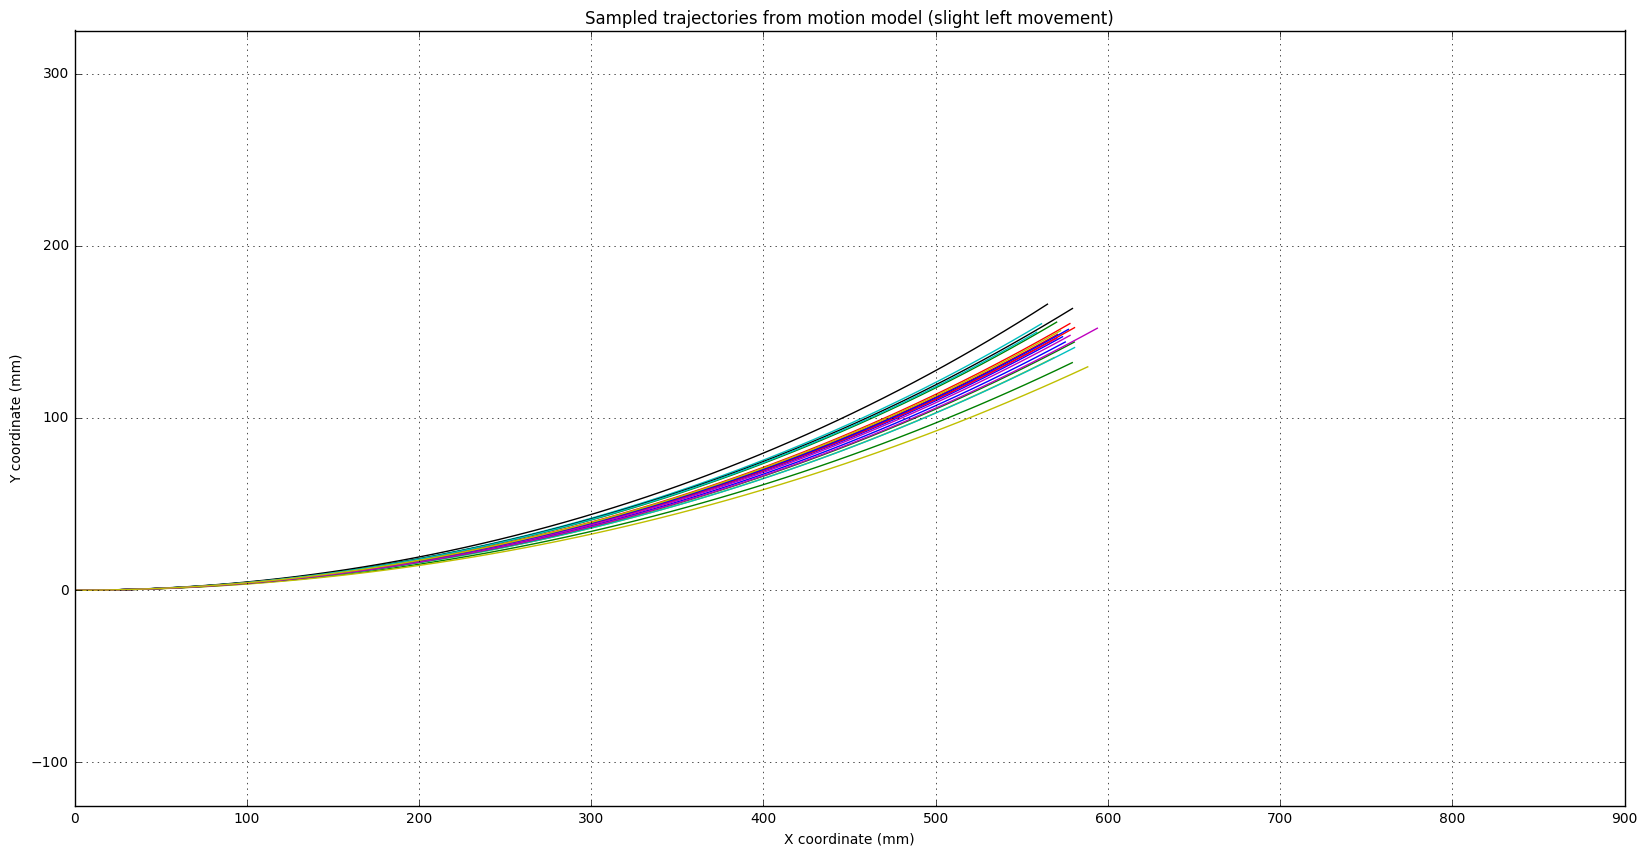
\includegraphics[width=1\textwidth]{images/sampled_poses_slightLeft.png} % second figure itself
        \caption{Sampled poses of the LeJOS robot going slight left.}
    \end{minipage}
    \end{figure}

    \begin{figure}[H]
        \centering
        \begin{minipage}{\textwidth}
            \centering
            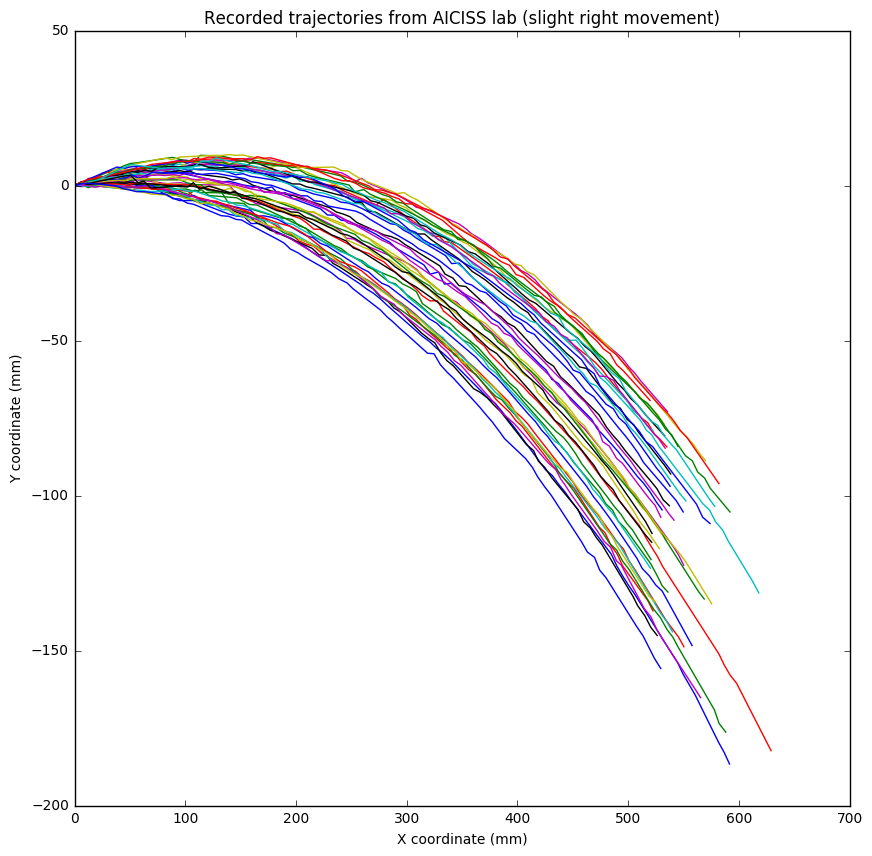
\includegraphics[width=1\textwidth]{images/recorded_poses_slight_right.png} % first figure itself
            \caption{Recorded poses of the LeJOS robot going slight right.}
        \end{minipage}\hfill
        \begin{minipage}{\textwidth}
            \centering
            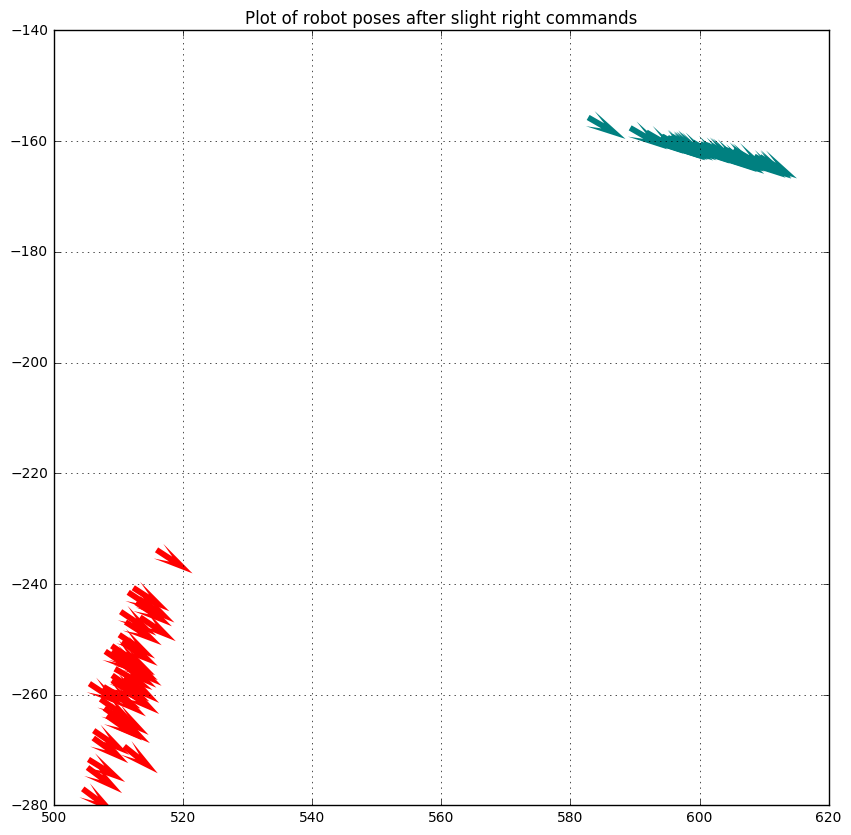
\includegraphics[width=1\textwidth]{images/sampled_poses_slightRight.png} % second figure itself
            \caption{Sampled poses of the LeJOS robot going slight right.}
        \end{minipage}
    \end{figure}

\begin{thebibliography}{9}
    \bibitem{Thrun}
    S. Thrun et al., “Velocity Motion Model,” in Probabilistic Robotics, ch. 5, pp. 121–132, Cambridge,
    MA: The MIT Press, 2006.
\end{thebibliography}
\end{document}
